
\label{cap_resultados}

\indent

Apresentamos neste capítulo a metodologia empregada e os resultados experimentais obtidos ao testar se fórmulas com menos cláusulas produzem respostas mais rápido e ao comparar algoritmos para escolha de renomeamento.

Os códigos-fonte e dados citados neste capítulo estão disponíveis no endereço\break \url{https://github.com/matheuscscp/TG}.

\section{Metodologia}

\indent

Apresentamos nesta seção os detalhes necessários para reproduzir os experimentos realizados.

\subsection{Representações de fórmulas}

\indent

A forma de representação de fórmulas lógicas utilizada em textos teóricos, ou seja, cadeias de uma determinada linguagem formal, complica bastante a tarefa de implementar transformações ou algoritmos de busca.

Observe, no entanto, que definimos a linguagem formal da lógica proposicional como uma \emph{gramática livre-do-contexto} \cite{sipser2012introduction} e, portanto, é garantido que existe um algoritmo de custo de tempo polinomial determinístico para obter a \emph{árvore sintática}, ou simplesmente \emph{árvore}, de uma fórmula \cite{younger1967recognition}. Tal estrutura se mostra muito mais prática para a implementação de algoritmos de transformação e busca do que cadeias de linguagens formais.

Ainda melhor que árvores para representar fórmulas, são \emph{grafos acíclicos dirigidos}, ou simplesmente DAGs na sigla do inglês. Em um DAG, qualquer subfórmula é representada por um único objeto \cite{jackson2004clause}, ou seja, mesmo que uma subfórmula ocorra em várias posições da fórmula principal, ela não é replicada para cada ocorrência. Tais estruturas equivalem a representar o conjunto de subfórmulas de fato como um conjunto, ou seja, $|\{\psi \in SFP(\phi) : \psi = \xi \}| = 1$, para todas $\phi$ e $\xi \sqsubseteq \phi$. É então uma forma de representação que se contrapõe a de uma árvore, que representa o conjunto de subfórmulas como um multiconjunto, ou seja, é possível acontecer $|\{\psi \in SFP(\phi) : \psi = \xi \}| > 1$. Em outras palavras, árvores sempre representam fórmulas como se nunca houvesse repetição de subfórmulas, criando cópias distintas para as distintas posições em que uma mesma subfórmula ocorre. Portanto, DAGs permitem uma representação mais fiel ao tratamento teórico dado neste trabalho, ou seja, múltiplas ocorrências de subfórmulas podem ser observadas na representação de uma fórmula. Além disso, DAGs são exponencialmente menores que árvores no melhor caso, como mostra a Figura \ref{figura_DAG}, e, portanto, propícios a algoritmos de programação dinâmica \cite{bellman2015applied} exponencialmente mais rápidos no melhor caso.

\begin{figure}
	\centering
	
	\raisebox{3.5\height}{$(p \leftrightarrow p) \leftrightarrow (p \leftrightarrow p)$}
	\hspace{1cm}
	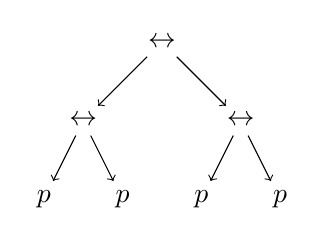
\begin{tikzpicture}
	\tikzset{vertex/.style = {}}
	\tikzset{edge/.style = {->}}
	
	\node[vertex]  (1) at (   0,    1) {$\leftrightarrow$};
	\node[vertex]  (2) at (  -1,    0) {$\leftrightarrow$};
	\node[vertex]  (3) at (   1,    0) {$\leftrightarrow$};
	\node[vertex]  (4) at (-1.5,   -1) {$p$};
	\node[vertex]  (5) at (-0.5,   -1) {$p$};
	\node[vertex]  (6) at ( 0.5,   -1) {$p$};
	\node[vertex]  (7) at ( 1.5,   -1) {$p$};
	
	\draw[edge] (1) to  (2);
	\draw[edge] (1) to  (3);
	\draw[edge] (2) to  (4);
	\draw[edge] (2) to  (5);
	\draw[edge] (3) to  (6);
	\draw[edge] (3) to  (7);
	\end{tikzpicture}
	\hspace{2cm}
	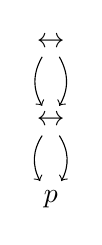
\begin{tikzpicture}
	\tikzset{vertex/.style = {}}
	\tikzset{edge/.style = {->}}
	
	\node[vertex]  (1) at (   0,    1) {$\leftrightarrow$};
	\node[vertex]  (2) at (   0,    0) {$\leftrightarrow$};
	\node[vertex]  (3) at (   0,   -1) {$p$};
	
	\draw[edge] (1) to [bend right] (2);
	\draw[edge] (1) to [bend left ] (2);
	\draw[edge] (2) to [bend right] (3);
	\draw[edge] (2) to [bend left ] (3);
	\end{tikzpicture}
	
	\hspace{1.45cm}(a)\hspace{4.2cm}(b)\hspace{3.85cm}(c)
	
	\label{figura_DAG}
	\caption{Representações de $(p \leftrightarrow p) \leftrightarrow (p \leftrightarrow p)$. (a) Cadeia. (b) Árvore. (c) DAG.}
\end{figure}

As três formas de representação de fórmulas apresentadas nesta seção são utilizadas em diferentes etapas da implementação, como discutimos a seguir.

\subsection{Implementação}
\label{impl}

\indent

Implementamos um programa, utilizando a linguagem de programação C++ versão 11 \cite{cpp11}, que recebe uma fórmula sob a forma de cadeia, realiza uma série de transformações e dá como saída uma fórmula resultante também sob a forma de cadeia, juntamente com três medidas desta última fórmula: seu tamanho, número de cláusulas e número de símbolos proposicionais. As transformações realizadas são detalhadas a seguir. Optamos por deixar flexível a execução ou não de algumas transformações, mas fixamos a ordem em que as transformações são realizadas.

\subsubsection{Análise sintática}

\indent

Convertemos uma fórmula sob a forma de cadeia para uma árvore sintática. Implementamos um algoritmo de pilha \cite{sipser2012introduction,CLRS09}, que faz uma única varredura na cadeia e produz a árvore. Esta transformação é sempre executada.

\subsubsection{Conversão para FNN}

\indent

A próxima transformação coloca a fórmula na forma normal negada. Esta etapa é feita através de uma busca em profundidade \cite{CLRS09}, onde o vértice pai é processado antes dos filhos, ou seja, em ordem \emph{prefixada}. Realizamos esta transformação por dois motivos em particular:
\begin{enumerate}
	\item As versões dos algoritmos para escolha de renomeamento e do algoritmo de conversão para a FNC são extremamente mais simples para fórmulas na FNN;
	\item Optando por não realizar a conversão para DAG mais adiante, a transformação que obtemos simula uma árvore linear. É claro que, em geral, as fórmulas não são necessariamente árvores lineares. No entanto, se for representada por uma árvore sintática, qualquer fórmula na FNN é considerada uma árvore linear pelos algoritmos de renomeamento, pois eles não conseguem identificar vértices distintos representando uma mesma subfórmula. Portanto, podemos testar casos em que os algoritmos não necessariamente escolhem renomeamentos ótimos, mas necessariamente escolhem renomeamentos que geram o mesmo número de cláusulas.
\end{enumerate}

Esta transformação é necessária somente para a realização de renomeamento e conversão para FNC. Pode ser desligada, caso o objetivo da execução do programa seja apenas obter as medidas da fórmula original.

\subsubsection{Aplainamento}

\indent

Aplicamos aplainamento à exaustão, também através de busca em profundidade prefixada. Isto não é necessário para nenhuma outra transformação e portanto pode-se optar por não realizar aplainamento. No entanto, esta transformação faz com que apareçam mais situações em que é possível aplicar simplificação \cite{sebastiani2009automated}. E, ainda, no contexto de renomeamento, o exemplo a seguir evidencia como aplainamento pode ser proveitoso.

Considere $\phi$ da forma $(p \wedge (q \wedge r)) \vee ... \vee ((p \wedge q) \wedge r)$. Na forma aplainada de $\phi$, $(p \wedge q \wedge r)$ pode ser renomeada por um único novo símbolo proposicional em suas duas ocorrências, se $\phi$ estiver representada por um DAG.

\subsubsection{Conversão para DAG}

\indent

A conversão é feita através de um algoritmo ascendente, ou seja, construímos o DAG de baixo para cima, indo das folhas até a raiz da árvore. Esta transformação não é necessária para nenhuma transformação seguinte e é possível optar por não executá-la.

Vale observar ainda que optamos por executar a conversão para DAG somente após colocar a fórmula na FNN, dado que isto evita o seguinte problema.

Suponha que $\psi$ ocorra em $\pi_1 \in pos(\phi)$ e em $\pi_2 \in pos(\phi)$ e suponha ainda que $pol(\phi,\pi_1) = 1 = -pol(\phi,\pi_2)$. Neste caso, é provável que, durante a conversão para FNN, $\psi$ deva ser transformada de duas maneiras distintas, uma em cada posição. Isto complicaria a conversão, caso a representação de $\phi$ fosse um DAG. Em uma árvore, no entanto, onde diferentes cópias de $\psi$ são criadas para diferentes posições em que $\psi$ ocorre, este problema é resolvido transparentemente.

\subsubsection{Renomeamento}

\indent

Nesta etapa, há três opções:
\begin{enumerate}
	\item Não realizar nenhum renomeamento;
	\item Aplicar o renomeamento escolhido pelo algoritmo de Boy de la Tour;
	\item Aplicar o renomeamento $f(n,n)$, que propomos e descrevemos no Capítulo \ref{cap_algoritmo}.
\end{enumerate}

Observamos a seguir os detalhes cruciais das implementações dos algoritmos de renomeamento.

Como dito anteriormente, ambos os algoritmos de renomeamento são implementados para fórmulas na FNN. Como na FNN só há negações na frente de símbolos proposicionais, temos que $$p(\psi) > 1 \implies b_\psi^\phi = 0, \forall \phi \in \mathcal{L} \text{ e } \psi \in SF(\phi)$$ Isto reduz a condição da Linha 4 do Algoritmo \ref{boydelatour}: $$a \cdot \psi.p > a + if\_pos(r,\psi.p) + if\_pos(-r,\psi.\overline{p})$$

Observe ainda que o valor de $r$, no Algoritmo \ref{boydelatour}, só deixa de ser 1 na Linha 11, quando $pol(\psi,i) \neq 1$. Mas, na FNN, ocorre que $$p(\phi|_\pi) > 1 \implies pol(\phi,\pi) = 1,\forall \phi \in \mathcal{L} \text{ e } \pi \in pos(\phi)$$ Logo, a condição da Linha 4 é reduzida mais uma vez: $$a \cdot \psi.p > a + \psi.p$$

Por fim, como é garantido que $\psi.p > 1$ quando a Linha 4 é executada, esta última condição se reduz novamente: $$a > 2 \text{ ou } (a = 2 \text{ e } \psi.p > 2)$$

Este último resultado nos permite implementar o algoritmo de Boy de la Tour sem aritmética de precisão arbitrária, pois, como as únicas operações aritméticas realizadas para calcular os valores de $a$ e $p$ são a adição e a multiplicação, podemos simplesmente truncar valores grandes para evitar que transbordamento aritmético ocorra. Acontece, no entanto, que este truncamento nos leva a outro problema.

Há duas alternativas para implementar o Algoritmo \ref{boydelatour} em sua complexidade correta (quadrática). A mais simples é calcular o produto $a_{\psi_i}^\phi = a \prod_{j} \psi_j.p$, utilizado na Linha 11, uma única vez e dividí-lo por $\psi_i.p$ apropriadamente em cada iteração do laço da Linha 10. Como optamos por uma representação numérica que não permite divisão, utilizamos uma segunda alternativa. Calculamos previamente uma tabela $dp$ que satisfaz\break $dp[i] = \prod_{j=i+1}^{n} \psi_j.p$, $i = 1,2,...,n$, e atualizamos o valor de $a$ a cada iteração com\break $a \gets a \cdot \psi_i.p$. Desta forma, o produto é corretamente calculado a cada iteração pela expressão $a \cdot dp[i]$. Nesta alternativa, nenhuma divisão é necessária.

Um detalhe adicional precisa ser considerado para a correção do método que utilizamos para calcular $a_{\psi_i}^\phi$. Observe que este valor precisa ser calculado a partir dos campos $\psi_j.p$. Acontece que, se a fórmula estiver representada por um DAG, o valor de $\psi_j.p$ poderia mudar durante a execução da chamada recursiva para $\psi_i$, para algum $j > i+1$, de modo que a tabela que calculamos previamente forneceria um valor incorreto para a iteração seguinte, quando $i$ passa a valer $i+1$. Evitamos este problema fazendo uma ordenação topológica nas arestas que saem de $\psi$, de modo que se $\psi_j \sqsubset \psi_k$, então $j < k$. Isto é de fato uma solução correta para o problema, porque qualquer DAG possui pelo menos uma ordenação topológica \cite{CLRS09}.

Na implementação do Algoritmo \ref{knapsack}, por outro lado, não utilizar aritmética de precisão arbitrária no cálculo de $p(\phi)$ levaria a resultados possivelmente incorretos. Assim, para que os resultados fossem corretos, e portanto no mínimo fiéis à heurística, optamos por implementar e utilizar aritmética de precisão arbitrária.

Por fim, é importante mencionar que, para calcular $f(n,n)$ através do Algoritmo \ref{knapsack}, a ordem de $SFP(\phi) = \{\phi_1,...,\phi_n \}$ é dada por uma busca em largura, ou seja, os primeiros vértices considerados pelo Algoritmo \ref{knapsack} estão mais perto da raiz.

\subsubsection{Conversão para FNC}

\indent

A última etapa do programa executa distribuição para colocar a fórmula na FNC e dá como saída a fórmula final sob a forma de cadeia. Esta etapa também é feita através de busca em profundidade prefixada. É possível ainda optar por não colocar a fórmula na FNC, ou ainda, durante a distribuição, aplicar as seguintes simplificações: eliminação de literais e cláusulas repetidos e eliminação de tautologias.

Escolhemos aplicar simplificação somente no final do programa, para que, justamente optando por não aplicar, fosse possível obter melhores comparações dos algoritmos de renomeamento. Não obstante, apresentamos resultados em que simplificação é aplicada.

\subsection{Experimentos propostos}

\indent

Para tentar responder às perguntas propostas, executamos o programa implementado para diversas combinações de transformações sobre um \textit{benchmark} tradicional de 1200 fórmulas intuicionistas \cite{raths07jar}. Optamos por utilizar este \emph{benchmark}, pois a maioria dos \emph{benchmarks} tradicionais apresentam fórmulas já em uma forma normal, ou possuem poucas fórmulas proposicionais, como o proposto por Sutcliffe \cite{sutcliffe09jar}. Portanto, com o \textit{benchmark} escolhido, pudemos testar nossas hipóteses de maneira mais exaustiva. Em seguida, executamos sobre as fórmulas transformadas o provador de teoremas E, um decisor para VAL baseado em forma normal clausal \cite{Schulz:LPAR-2013}. Foram anotadas as medidas de cada fórmula fornecidas ao final da etapa de pré-processamento, os tempos de execução nas duas etapas e o resultado do decisor de validade.

As dez combinações de transformações testadas são descritas na Tabela \ref{combinacoes}. Em cada combinação, executamos um subconjunto das transformações apresentadas na Seção \ref{impl}. Na tabela, a presença de um X indica que a transformação da respectiva linha foi executada na combinação da respectiva coluna. Uma célula vazia indica que a respectiva transformação não foi executada na respectiva combinação. Na linha de renomeamento, o número 1 indica que o algoritmo de renomeamento executado é o proposto por Boy de la Tour (Algoritmo \ref{boydelatour}), enquanto o número 2 indica que o algoritmo executado é o que propomos neste trabalho (Algoritmo \ref{knapsack}). Finalmente, na linha de conversão para FNC, o número 1 indica que foi executada somente distribuição, enquanto o número 2 indica que foi executada distribuição com simplificação.

\tabela{Combinações de transformações executadas}{combinacoes}{l|cccccccccc}{
	Combinação         & 1 & 2 & 3 & 4 & 5 & 6 & 7 & 8 & 9 & 10 \\ \hline
	Análise sintática  & X & X & X & X & X & X & X & X & X & X  \\
	Conversão para FNN & X & X & X & X & X & X & X & X & X & X  \\
	Aplainamento       & X & X & X & X & X & X & X & X & X & X  \\
	Conversão para DAG &   &   &   &   &   &   & X & X & X & X  \\
	Renomeamento       &   &   & 1 & 1 & 2 & 2 & 1 & 1 & 2 & 2  \\
	Conversão para FNC & 1 & 2 & 1 & 2 & 1 & 2 & 1 & 2 & 1 & 2  \\
}

Os experimentos foram executados em um computador com sistema operacional\break Ubuntu 14.04 (GNU/Linux 3.19.0-30-generic x86\_64), processador Intel\textsuperscript{\textregistered} Xeon\textsuperscript{\textregistered}\break Processor E5-2620 v3, que possui frequência de \textit{clock} 2.4GHz e 15M de memória\break \textit{cache}, e memória RAM de 64GiB. Cada combinação foi executada com um limite máximo de 4GB de memória virtual, tamanho ilimitado para o segmento de pilha e mil segundos de limite de tempo.

\section{Resultados e análise}

\indent

Dos dados coletados, foi feita uma análise exaustiva. Apresentamos nesta seção os principais destaques.

\subsection{Combinações sem renomeamento}

\indent

Primeiro, observamos os resultados das Combinações 1 e 2, onde não foi feito nenhum renomeamento e alternamos somente entre aplicar ou não simplificação durante a etapa de distribuição.

Na Combinação 1, onde simplificação não foi aplicada, 73\% das fórmulas excederam o limite de memória na etapa de pré-processamento e o restante foi transformado com sucesso. Na Combinação 2, 67\% excedeu o limite de memória e 1\% excedeu o limite de tempo. Além disso, dos 27\% em que todas as fórmulas foram transformadas com sucesso por ambas as combinações, 5 fórmulas (menos de 1\%) ficaram com o mesmo tamanho, enquanto todas as restantes ficaram menores ao aplicar simplificação. Isto faz bastante sentido, pois se uma fórmula contém exatamente $n$ símbolos proposicionais distintos, então:
\begin{enumerate}
	\item Ao eliminar literais repetidos e tautologias, cada cláusula gerada pela fórmula pode conter no máximo $n$ literais.
	\item Ao eliminar cláusulas repetidas, a fórmula pode gerar no máximo $3^n$ cláusulas distintas. Isto ocorre porque, para cada símbolo proposicional e uma cláusula fixa sem tautologias e literais repetidos, há somente três possibilidades: ou o símbolo não ocorre na cláusula, ou ele ocorre, ou ele ocorre negado.
\end{enumerate}
Em outras palavras, uma fórmula com as simplificações que aplicamos possui um tamanho máximo ao ser convertida para a FNC.

A observação principal é que apenas simplificação não é suficiente para obter bons resultados, já que mais da metade das fórmulas sequer pôde ser pré-processada com sucesso dentro das restrições de tempo e memória utilizadas.

\subsection{Testando a conjectura para árvores lineares}

\indent

Das Combinações 3 e 5, que aplicam a árvores respectivamente os Algoritmos \ref{boydelatour} e \ref{knapsack} para escolha de renomeamento e não aplicam simplificação durante a etapa de distribuição, obtemos uma amostra da correção da Conjectura \ref{conjectura} (optimalidade do Algoritmo \ref{knapsack} para árvores lineares). Como discutido na Seção \ref{impl}, estas combinações \emph{simulam} árvores lineares e, portanto, sob essa condição, não necessariamente os Algoritmos \ref{boydelatour} e \ref{knapsack} devem encontrar renomeamentos que geram o menor número possível de cláusulas para uma fórmula qualquer, mas ambos devem encontrar renomeamentos que geram exatamente o mesmo número de cláusulas para esta fórmula. Para todas as fórmulas que puderam ser transformadas com sucesso em ambas as combinações (49\%), constatamos esta propriedade. Além disso, nenhuma fórmula excedeu o limite de memória somente na Combinação 5. Caso ocorresse, esta situação seria um leve indício de que a conjectura talvez não fosse válida. Estes dois fatos indicam fortemente que a Conjectura \ref{conjectura} provavelmente é um teorema.

\subsection{Comparações entre árvores e DAGs}
\label{secao_tree_x_dag}

\indent

Comparamos agora os resultados das Combinações de 3 a 6, onde a estrutura de representação utilizada foi árvore, com as Combinações de 7 a 10, onde a estrutura utilizada foi DAG, ou seja, comparamos cada combinação com sua igual, a menos do tipo de representação utilizada. Portanto, referindo-nos à Combinação $i$ abreviadamente por $C_i$, comparamos $C_i$ (árvore) com $C_{i+4}$ (DAG), para $i=3,4,5,6$.

O primeiro resultado observado, que é relativo ao número de cláusulas produzido em cada combinação, é apresentado na Tabela \ref{dag_x_tree_info}. As seguintes regras foram usadas para determinar quando cada representação foi melhor. Para uma fórmula fixa $\phi$, $C_i$ foi melhor que $C_{i+4}$ se, e somente se:
\begin{enumerate}
	\item ambas $C_i$ e $C_{i+4}$ transformaram $\phi$ com sucesso, isto é, não excederam o limite de tempo ou memória, e a transformação produzida por $C_i$ gera menos cláusulas que a transformação produzida por $C_{i+4}$; ou
	\item $C_i$ transformou $\phi$ com sucesso e $C_{i+4}$ não.
\end{enumerate}
O critério análogo obtido trocando cada ocorrência de $C_i$ por $C_{i+4}$ e vice-versa foi utilizado para determinar quando $C_{i+4}$ foi melhor que $C_i$.

\tabela{Árvore $\times$ DAG. Número de cláusulas}{dag_x_tree_info}{l|c|c|c|c|l}{
	& $C_3 \times C_7$ & $C_4 \times C_8$ & $C_5 \times C_9$ & $C_6 \times C_{10}$ \\ \hline
	$C_i$ foi melhor em & 0 (0\%)     & 5 (0\%)     & 0 (0\%)     & 6 (1\%)      & fórmulas. \\
	$C_{i+4}$ foi melhor em    & 179 (15\%)  & 177 (15\%)  & 367 (31\%)  & 358 (30\%)   & fórmulas. \\
}

Da Tabela \ref{dag_x_tree_info}, note que as combinações com representação por DAG, em geral, produziram fórmulas com menos cláusulas. Observe ainda que nos pares onde simplificação não é aplicada ($C_3 \times C_7$ e $C_5 \times C_8$), nenhuma fórmula gerou menos cláusulas na transformação por $C_i$ (árvore). Estes fatos fazem bastante sentido, pois, do ponto de vista de algoritmos de renomeamento, a única diferença entre as duas formas de representação é que DAGs permitem que todas as ocorrências de uma mesma subfórmula sejam renomeadas por um único novo símbolo proposicional. Note que mesmo aplicando simplificação ao final das transformações (pares $C_4 \times C_8$ e $C_6 \times C_{10}$), DAGs ainda geram menos cláusulas em grande parte das vezes.

Em segundo lugar, observamos o tempo de execução da etapa de pré-processamento. Os resultados são apresentados no gráfico da Figura \ref{dag_x_tree_time}. Cada ponto sobre o eixo horizontal identifica uma das 1200 fórmulas do \textit{benchmark}. O eixo vertical é o tempo de $C_i$ menos o tempo de $C_{i+4}$, em segundos. Do gráfico, nota-se que a maior parte das diferenças é positiva e com um grande valor absoluto. Isto quer dizer que, na maior parte das vezes, DAGs obtiveram melhor desempenho durante a etapa de pré-processamento. O que não é surpresa, pois, mesmo que $C_{i+4}$ não gere menos cláusulas, algoritmos de transformação executam mais rápido em representações mais compactas.

\figura[]{arvore_x_dag_time}{Árvore X DAG. Tempo de pré-processamento}{dag_x_tree_time}{}

Por último, analisamos o tempo de execução na etapa de busca, ou seja, o tempo de execução do provador E. O gráfico da Figura \ref{dag_x_tree_ptime}, que ilustra estes resultados, foi construído de maneira similar ao gráfico da Figura \ref{dag_x_tree_time}, ou seja, cada ponto no eixo horizontal representa uma fórmula e cada altura indica a diferença entre o tempo medido para $C_i$ e o tempo medido para $C_{i+4}$. Mais uma vez, notamos que a maior concentração de pontos está acima ou sobre o eixo horizontal de diferença igual a zero. E, novamente, isto indica que, em grande parte das vezes, DAGs obtiveram melhor desempenho, mas agora na etapa de busca.

Com esta última observação, temos o primeiro indício de que, muitas vezes, fórmulas com menos cláusulas podem produzir respostas mais rápido. Esta conclusão é bastante razoável, já que, como observamos antes, a principal diferença entre as fórmulas produzidas por cada um dos dois grupos de combinações é justamente o número de cláusulas, que é menor para DAGs em grande parte das vezes.

Com os resultados apresentados nesta seção, há um forte indício de que, independentemente dos resultados de optimalidade restrita dos algoritmos de renomeamento serem para árvores lineares, é melhor realizar conversão para DAG na grande maioria das vezes. Portanto, a partir de agora, voltamos nossa atenção para comparações envolvendo somente combinações que realizam conversão para DAG.

\figura[]{arvore_x_dag_ptime}{Árvore X DAG. Tempo de busca}{dag_x_tree_ptime}{}

\subsection{Comparações entre os algoritmos de renomeamento}

\indent

O primeiro resultado que observamos é bastante surpreendente e animador. Comparamos as Combinações 7 e 9, que aplicam a DAGs respectivamente os Algoritmos \ref{boydelatour} e \ref{knapsack}, sem aplicar simplificação ao final. No total, 73\% das fórmulas foram transformadas com sucesso por ambas as combinações. Ocorre ainda que 3\% das fórmulas foram transformadas com sucesso e a combinação com o algoritmo de Boy de la Tour produziu menos cláusulas, com diferença máxima de 3 cláusulas. Antes de mais nada, isto prova que o algoritmo que propomos não encontra renomeamentos ótimos para qualquer fórmula. Por outro lado, 8\% das fórmulas foram transformadas com sucesso e, além disso, a combinação com o algoritmo que propomos produziu menos cláusulas. Desta vez, a diferença máxima chegou a 1.572.786 cláusulas, onde a fórmula produzida por nosso algoritmo gera apenas 78 cláusulas. Primeiro, isto prova que o algoritmo de Boy de la Tour também não encontra renomeamentos ótimos para qualquer fórmula. Mas este resultado também indica que o algoritmo que propomos, apesar de possuir a complexidade do algoritmo de Boy de la Tour multiplicada por um fator linear, pode produzir renomeamentos que geram muito menos cláusulas para algumas fórmulas.

Estes resultados ocorrem dentro de famílias de fórmulas específicas. O algoritmo de Boy de la Tour produziu menos cláusulas somente na família de fórmulas \emph{nishimura}. O algoritmo que propomos produziu menos cláusulas principalmente nas famílias \emph{SYJ205}, \emph{SYJ206} e \emph{SYJ212}. As diferenças mais discrepantes ocorrem nas famílias \emph{SYJ206} e \emph{SYJ212}, onde o algoritmo que propomos é capaz de encontrar subfórmulas em níveis mais altos para renomear, enquanto o algoritmo de Boy de la Tour não é. Observando ainda os resultados das combinações análogas que aplicam simplificação ao final, notamos que os resultados são semelhantes, apenas trocando as famílias em que as diferenças são pequenas e mantendo as famílias onde as diferenças são maiores.

\figura[]{boy_x_knapsack_ptime}{Boy de la Tour X Algoritmo proposto. Tempo de busca}{boy_x_knapsack_ptime}{}

Por último, comparamos os desempenhos das transformações produzidas pelos algoritmos de renomeamento durante a etapa de busca.

O gráfico da Figura \ref{boy_x_knapsack_ptime} foi construído similarmente aos gráficos da Seção \ref{secao_tree_x_dag}. O eixo horizontal identifica as fórmulas, enquanto o eixo vertical é a diferença entre o tempo de busca de $C_i$ (Boy de la Tour) e $C_{i+2}$ (algoritmo proposto), para $i=7,8$. Do gráfico, observamos que as concentrações de pontos acima e abaixo do eixo horizontal de diferença igual a zero são bastante parecidas, no sentido de que um algoritmo leva vantagem em algumas famílias de fórmulas, enquanto o outro leva vantagem em outras.

\subsection{Tempo de busca em função do número de cláusulas}

\figura[]{ptime}{Tempo de busca em função do número de cláusulas}{ptime}{width=0.7\textwidth}

\figura[]{ptime_SYJ}{Tempo de busca em função do número de cláusulas. Família \emph{SYJ206}}{ptime_SYJ}{width=0.7\textwidth}

\indent

Finalmente, tentamos responder à pergunta inicial. O gráfico da Figura \ref{ptime} é o tempo de busca em função do número de cláusulas. Neste gráfico, incluímos todas as execuções feitas com sucesso. Como algumas transformações geraram o mesmo número de cláusulas, há múltiplos pontos em diversas posições ao longo do eixo horizontal. Do gráfico, notamos que o comportamento do tempo de busca em função do número de cláusulas não é estritamente crescente ou suave. Ora, curiosa seria a realidade em que esta relação funcional fosse de fato tão bem comportada. No entanto, é sim notável um certo grau de bom comportamento crescente em diversas partes do gráfico, que se misturam. E, muito provavelmente, isto ocorre dentro de cada família de fórmulas do \emph{benchmark}, como mostra o gráfico da Figura \ref{ptime_SYJ}, feito exclusivamente para a família \emph{SYJ206}. Portanto, uma conclusão razoável é que, considerando fórmulas similares, sim, as com menos cláusulas produzem respostas mais rápido em algoritmos de busca.
